La nouvelle méthode de traitement des homographies repose sur la décomposition d'une homographie qui permet d'interpréter cette dernière en terme de mouvement de caméra. La partie ci-dessous présente cette décomposition.

\ssse{Mouvement de caméra}
\label{mouv_de_camera}
On étudie ici un cas a priori particulier d'homographie $h$ : les homographies que l'on peut interpréter comme un mouvement de caméra idéale. On montrera par la suite que c'est en fait un cas général.

Nous modéliserons la situation en supposant que la scène filmée est plane. Cela suppose que l'on filme une surface soit sans aucun relief, soit avec un relief négligeable devant la distance à la caméra, afin qu'il ne soit pas perceptible. La figure \ref{shmdecomp} illustre la modélisation utilisée pour la caméra idéale, les paramètres introduits sur ce schéma seront définis dans les définitions et notations \ref{defpoint}. La caméra idéale se modélise donc par la projection d'un plan sur un autre en passant par un foyer $F$, en négligeant les lentilles ou les dispositifs correcteurs présents dans les caméras réelles.
\begin{figure}[h!]

\centering
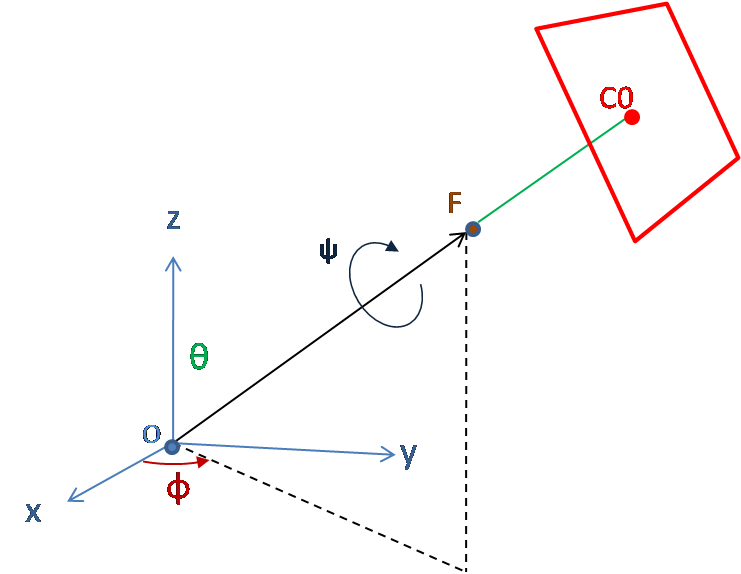
\includegraphics[width=10cm]{shema_decomp.png}
\caption{Illustration d'un mouvement de caméra $(X_v =0)$ (les translations ont été omises pour plus de clarté. $F$ représente le point focal de la caméra, le plan rouge est le plan image de la caméra. Un point du plan image est le projeté passant par $F$ d'un point du plan $(x,y)$. (cf. partie \ref{mouv_de_camera})}
\label{shmdecomp}
\end{figure}

\begin{defnot}
On se place dans l'espace $\mathbb{R}^{3}$, on le munit d'une base orthonormée directe $(\xbf_0,\ybf_0,\zbf_0)$.

L'image de départ sera située dans le plan $P_{1}= \mathbb{R}^{2}\times \{0\}$.

On doit maintenant positionner notre caméra par rapport à l'image de départ (figure \ref{shmdecomp}).

\begin{itemize}
\item On note $F$ la position de l'objectif de la caméra, et $\wbf$ le vecteur directeur unitaire de l'axe optique de la caméra. L'axe optique de la caméra est donc la droite passant par $F$ et dirigée par $\wbf$.

\item On note $\delta$ la distance entre l'objectif et l'écran.

\item L'écran $P_{2}$ est alors le plan affine passant par $F+\delta \wbf$ et perpendiculaire à l'axe optique de la caméra.
\begin{equation*}
P_{2}=\{Y\in \mathbb{R}^{3}|(Y-F-\delta \wbf)\cdot \wbf=0\}=\{Y\in \mathbb{R}^{3}|(Y-F)\cdot \wbf=\delta\}
\end{equation*}

\item Si on se place dans le cas où le vecteur $\wbf$ n'appartient pas à $P_{1}$, on peut alors définir $X_{v}$ le point de $P_{1}$ visé par la caméra, c'est-à-dire le point d'intersection entre l' axe optique et le plan $P_{1}$. On obtient alors
\begin{equation*}
X_{v}=F-\delta'\wbf \text{ et }\delta'=\small{\left|\frac{F \cdot \zbf_{0}}{\wbf \cdot \zbf_{0}} \right|}
\end{equation*}

\item La caméra peut aussi effectuer une rotation autour de son axe optique, que l'on appellera rotation propre et dont l'angle sera noté $\psi$.
\end{itemize}

On définit l'application $H$ qui à un point $X\in P_{1}$ lui associe sa projection homographique sur $P_{2}$ (le point $H(X)$ est le point d'intersection de la droite $D_{X}$ passant par $X$ et $F$ et du plan $P_{2}$). Cette intersection n'existe pas toujours, le domaine de définition de $H$ est donc $P_1$ privé d'une droite $D$ qui correspond à un angle mort de la caméra.
\begin{equation*}
D=\{X\in P_1 | (X-F) \cdot \wbf =0\}
\end{equation*}

De même, l'image de $H$ est $P_2 \setminus D'$ où $D'$ est appelée l'horizon (du mouvement de caméra).
\begin{equation*}
D'=\{ X\in P_2 | (X-F).\zbf_0=0\}
\end{equation*}

On appelle $H:P_1 \setminus D \ra P_2 \setminus D'$ un mouvement de caméra.

Un mouvement de caméra est donc défini en fonction de $9$ paramètres, il n'y a pas unicité de ces paramètres.

Le plan $P_1$ sera muni du repère orthonormé $(0,\xbf_0,\ybf_0)$ ; le plan $P_{2}$ peut être muni d'un repère orthonormé $(C,u,v)$ tel que la famille $(\ubf,\vbf,\wbf)$ soit un base orthonormée directe de $\mathbb{R}^{3}$.

La base $(\ubf,\vbf)$ est définie en fonction des rotations effectuées par la caméra (son expression sera précisée plus tard). Le point $C$ est un point arbitraire de $P_2$, on ne cherchera pas à vérifier la condition $C=C_0$.

Par abus de notation, on note encore $D$ et $D'$ les droites de $\mathbb{R}^{2}$ lorsque l'on munit $P_1$ et $P_2$ des repères $(0,\xbf_0,\ybf_0)$ et $(C,\ubf,\vbf)$.

On peut repérer le point $C$ par rapport au centre de l'écran $C_{0}$, c'est-à-dire la projection orthogonale de l'objectif sur l'écran : $C_{0}=Z+\delta \wbf$ et $C=C_{0}+c^{u}\ubf+c^{v}\vbf$, où on note $\cbf=(c^u,c^v)$ et $\xbf_v = (X_v \cdot \xbf_0,X_v \cdot \ybf_0)$.

On définit enfin $h:\mathbb{R}^{2} \setminus D \ra \mathbb{R}^{2}\setminus D'$, qui, à $(x,y)$ coordonnées de $X\in P_1\setminus D$, associe $h(x,y)$ les coordonnées du point $H(X)\in P_2 \setminus D'$, dans $(C,\ubf,\vbf)$.
\label{defpoint}
\end{defnot}

\begin{remarque}
L'application $H$ est une bijection de $P_1 \setminus D$ dans $P_2 \setminus D'$ et $H^{-1}$ est aussi un mouvement de caméra

De plus, l'horizon de $H^{-1}$ est l'angle mort de $H$ et l'angle mort de $H^{-1}$ est l'horizon de $H$.
\end{remarque}

\begin{remarque}
L'application $H$ est une formulation géométrique du mouvement de caméra, et $h$ en est la formulation analytique.

On verra plus tard que $h$ est une homographie : c'est l'homographie associée au mouvement de caméra.
\end{remarque}

Dans la suite de cette section on fixe un jeux de paramètres $(\theta,\phi,\psi,\delta,\delta',\cbf,Z)$ et on considère le mouvement de caméra $H$ associé à ces paramètres.
Dans cette partie, on cherche à établir la décomposition suivante
\begin{prop}
 Soit  $H$ un mouvement de caméra de paramètres $(\theta,\phi,\psi,\delta,\delta',\cbf,Z)$,l'application $h$ est une homographie.
 De plus si  $H$ admet un point visé $X_v$ alors $h$ se factorise sous la forme
\begin{equation}
h = \tau_{\cbf_v} \circ z_{\frac{\delta}{\delta'}}  \circ R_{\psi} \circ h_{\theta,\delta'} \circ R_{\phi} \circ \tau_{\xbf_v}
\label{formul_decomp}
\end{equation}
Où $R_{\alpha}$ est la rotation d'angle $\alpha$,$z_\lambda$ est la dilatation de facteur $\lambda$, $\tau_\ybf$ est  la translation du vecteur $-\ybf$ et $h_{\theta,\delta'}$ est l'homographie unidirectionnelle (cf. définition \ref{homo_uni_direc})
\begin{equation}
h_{\theta,\delta'}(x',y')=\left(\frac{-cos(\theta)x'}{1-\frac{sin(\theta)}{\delta'}x'} ,\frac{-y'}{1-\frac{sin(\theta)}{\delta'}x'}\right)
\label{mise_perspective}
\end{equation}
\label{prop_decomp}
\end{prop}

\begin{Def}
Une homographie unidirectionnelle est une application $h:\mathbb{R}^{2} \ra \mathbb{R}^{2}$ définie par 
\begin{equation*}
h(x,y)=\left ( \frac{ax+p}{rx+t} , \frac{cy+p}{rx+t} \right)
\end{equation*}
Où $a,p,c,q,r,t$ sont des réels.
\label{homo_uni_direc}
\end{Def}

Le résultat de la proposition \ref{prop_decomp} est intuitif et se comprend facilement grâce à la figure \ref{shmdecomp}. Afin de le démontrer, on commencera par établir deux lemmes.

\begin{lem}Si le point visé $X_v$ existe alors
$\forall X \in P_1 \setminus D$
\begin{equation}
H(X)=Z+\delta \wbf+\delta \frac{(X_v-X)-\left((X_v-X)\cdot \wbf \right) \wbf}{\wbf \cdot (X_v-X)+\delta'}
\label{homo_form_geo}
\end{equation}
\end{lem}

\begin{proof}
On sait que $H(X)$ est le point d'intersection entre la droite $D_X$ passant par $X$ et $F$ , et le plan $P_2$.
Comme $D_{X}=\{X+t(F-X)|t\in\mathbb{R}\}$, si $H(X)$ existe alors 
\begin{equation*}
\exists t_{X},H(X)=X+t_{X}(F-X)
\end{equation*}
Comme $H(X)\in P_{2}$ alors
\begin{equation*}
(H(X)-F)\cdot \wbf =\delta
\end{equation*}
Et donc 
\begin{equation*}
t_{X}=1+\frac{\delta}{\wbf \cdot(F-X)}
\end{equation*}
 On en déduit que l'application $H$ est bien définie sur $P_{1}\setminus D$ et 
\begin{equation*}
H(X)=Z+\delta \wbf+\delta \frac{(F-X)-\left((F-X)\cdot \wbf \right) \wbf}{\wbf \cdot (F-X)}
\end{equation*}
Si le point visé $X_v$ existe alors  $F=X_v+\delta' \wbf$ et donc
\begin{equation*}
H(X)=Z+\delta \wbf+\delta \frac{(X_v-X)-\left((X_v-X)\cdot \wbf \right) \wbf}{\wbf \cdot (X_v-X)+\delta'}
\end{equation*}
\end{proof}
Afin de simplifier les expressions dans les calculs qui suivent on définit la bijection $i$ 
\begin{equation*}
i:\mathbb{R}^{2}\rightarrow P_{1},~~~~~~i((x,y))=x\xbf_{0}+y\ybf_{0}
\end{equation*}

\begin{lem}Si le point visé $X_v$ existe alors $\forall (x,y)\in \mathbb{R}^{2} \setminus D$ 
\begin{equation}
h((x,y))=\left(\frac{\delta (X_{v}-X)\cdot \ubf}{\wbf \cdot (X_v-X))+\delta'}-c^u,\frac{\delta (X_v-X)\cdot \vbf}{\wbf \cdot (X_v-X)+\delta'} -c^v \right) 
\label{homo_form_analytique}
\end{equation}
où $X=i(x,y)$
\end{lem}
Ce lemme montre en particulier que $h$ est bien une homographie.
\begin{proof}
Par définition de $h$,les composantes de $h((x,y))$ sont les coordonnées de $H(X)$ dans le repère orthonormé $(C,\ubf,\vbf)$ de $P_2$ (cf. définitions et notations \ref{defpoint}), on a donc $ \forall (x,y)\in \mathbb{R}^{2} \setminus D$
\begin{eqnarray*}
h((x,y)) &=& ((H(X)-C)\cdot \ubf, (H(X)-C)\cdot \vbf)\\
     &=& ((H(X)-Z-\delta -c^u \ubf -c^v \vbf)\cdot \ubf, (H(X)-Z-\delta -c^u \ubf -c^v \vbf)\cdot \vbf)\\
     &=& ((H(X)-Z)\cdot \ubf -c^u, (H(X)-Z)\cdot \vbf - c^v)
\end{eqnarray*}
Grâce à la formule du lemme précédent (formule \ref{homo_form_geo}) on en déduit alors 
\begin{equation*}
h((x,y))=\left(\frac{\delta (X_v-X)\cdot \ubf}{\wbf \cdot (X_v-X))+\delta'}-c^u,\frac{\delta (X_v-X)\cdot \vbf}{\wbf \cdot (X_v-X)+\delta'} -c^v \right) 
\end{equation*}
\end{proof}

On peut maintenant établir la formule de décomposition (formule \ref{formul_decomp}) de la proposition \ref{prop_decomp} ; les notations utilisées dans cette preuve ont été introduites au début de cette section (cf. définitions et notations \ref{defpoint}).

\begin{proof}
On peut positionner le vecteur $\wbf$ par rapport à la $(\xbf_{0},\ybf_{0},\zbf_{0}) $ en introduisant deux angles, $\phi$ et $\theta$.

\begin{itemize}
\item la première rotation d'angle $\phi$ se fait autour de l'axe $(0,\zbf_{0})$ ; on lui associe la base $(\xbf_{1},\ybf_{1},\zbf_{1}) $ où $\zbf_{0}=\zbf_{1}$.
\item la seconde rotation d'angle $\theta$ se fait autour de l'axe $(0,\ybf_1)$ ; on lui associe la base $(\xbf_{2},\ybf_{2},\zbf_{2}) $ où $\zbf_{2}=\wbf$ et $\ybf_{1}=\ybf_{2}$.
\end{itemize}

\begin{figure}[h!]
\centering
\subfigure[rotation d'angle $\phi$]{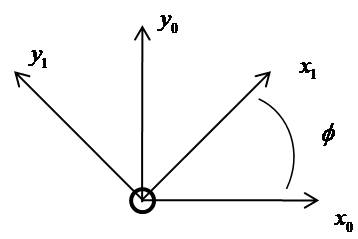
\includegraphics[width=5cm]{graphe1.jpg}}
\subfigure[rotation d'angle $\theta$]{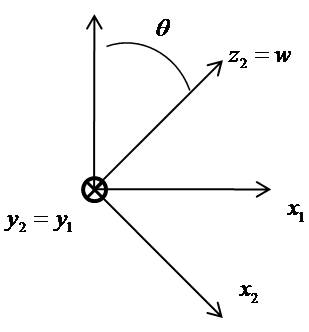
\includegraphics[width=5cm]{graphe2.jpg}}
\caption{(cf partie \ref{figure_de_rotations_18})}
\label{img_angles}
\end{figure}

Pour positionner la caméra, on doit définir sa rotation propre autour de son axe optique. Pour cela on définit l'angle $\psi$ (figure \ref{decompgeo_rotationPropre}).
\begin{figure}[h!]
\centering
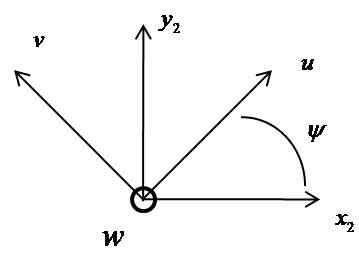
\includegraphics[width=5cm]{graphe3.jpg}
\caption{rotation propre (cf partie \ref{figure_de_rotations_18})}
\label{decompgeo_rotationPropre}
\end{figure}

On obtient alors
\begin{equation*}
\ubf=\cos(\psi)\xbf_{2}+\sin(\psi)\ybf_{2} \text{ et } \vbf=-\sin(\psi)\xbf_{2}+\cos(\psi)\ybf_{2}
\end{equation*}
Si on pose $R_{s}$ la rotation d'angle $s$ et $\tau_{\ybf}$ la translation de vecteur $-\ybf$, on obtient alors grâce au lemme précédent (formule \ref{homo_form_analytique})
\begin{eqnarray*}
(\tau_{\cbf}^{-1} \circ h)((x,y)) &=& \left(\frac{\delta (X_v-X)\cdot \ubf }{\wbf \cdot (X_v-X)+\delta'},\frac{\delta (X_v-X)\cdot \vbf}{\wbf \cdot (X_v-X)+\delta'}  \right) \\
                           &=& R_{\psi}\left(\frac{\delta (X_v-X)\cdot \xbf_{2} }{\wbf \cdot (X_v-X)+\delta'},\frac{\delta (X_v-X)\cdot \ybf_{2}}{\wbf \cdot (X_v-X)+\delta'}  \right) \\
\end{eqnarray*}
où on note toujours $X = i((x,y))$.

Comme $X_{v}=i(\xbf_v)$ on obtient
\begin{equation*}
(R_{\psi}^{-1} \circ \tau_{\cbf}^{-1}  \circ h)((x,y))=\delta \left(\frac{-i(\tau_{\xbf_v} ((x,y)))\cdot \xbf_{2} }{-\wbf \cdot i(\tau_{\xbf_v} ((x,y)))+\delta'},\frac{-i(\tau_{\xbf_v} ((x,y)))\cdot \ybf_{2}}{-\wbf \cdot i(\tau_{\xbf_v} ((x,y)))+\delta'}  \right) 
\end{equation*}

Comme $\zbf_{2}=cos(\theta)\zbf_{1}+sin(\theta)\xbf_{1}$, $\xbf_{2}=cos(\theta)\xbf_{1}-sin(\theta)\zbf_{1}$ (figure \ref{img_angles}) et $\zbf_{1}\perp P_{1}$, on a

\begin{equation*}
(R_{\psi}^{-1} \circ \tau_{\cbf}^{-1}  \circ h)((x,y))=\delta\left(\frac{-\cos(\theta)i(\tau_{\xbf_v} ((x,y)))\cdot \xbf_{1} }{\delta'-\frac{sin(\theta)}{\delta'}\xbf_{1}\cdot i(\tau_{\xbf_v}((x,y)))}, \frac{-i(\tau_{\xbf_v} ((x,y)))\cdot \ybf_{1}}{\delta'-\frac{sin(\theta)}{\delta'}\xbf_{1}\cdot i(\tau_{\xbf_v}((x,y)))}  \right) 
\end{equation*}

En définissant $h_{\theta,\delta'}$ par

\begin{equation*}
h_{\theta,\delta'}(x',y')=\left(\frac{-\cos(\theta)x'}{1-\frac{\sin(\theta)}{\delta'}x'} ,\frac{-y'}{1-\frac{\sin(\theta)}{\delta'}x'}\right)
\end{equation*}

Alors 

\begin{equation*}
(R_{\psi}^{-1} \circ \tau_{\cbf}^{-1} \circ h)((x,y))= \frac{\delta}{\delta'}h_{\theta,\delta'}\left ( i(\tau_{\xbf_v}((x,y))) \cdot \xbf_{1}, i(\tau_{\xbf_v}((x,y))) \cdot \ybf_{1}\right)
\end{equation*}
\label{figure_de_rotations_18}
Comme $\xbf_{1}=\cos(\phi)\xbf_{0}+\sin(\phi)\ybf_{0}$ et $\ybf_{1}=-\sin(\phi)\xbf_{0}+\cos(\phi)\ybf_{0}$ (figure \ref{img_angles}), alors

\begin{eqnarray*}
(R_{\psi}^{-1} \circ \tau_{\cbf}^{-1} \circ h)((x,y)) &=& \frac{\delta}{\delta'}h_{\theta,\delta'}\left ( R_{\phi}(i(\tau_{\xbf_v}((x,y))) \cdot \xbf_{0}, i(\tau_{\xbf_v}((x,y))) \cdot \ybf_{0})\right)\\
                                               &=&\frac{\delta}{\delta'} (h_{\theta,\delta'}\circ R_{\phi} \circ \tau_{\xbf_v})((x,y))
\end{eqnarray*}

Si on définit les dilatations $z_{\lambda}:X\rightarrow \lambda X$, alors on obtient la formule générale pour les mouvements de caméra

\begin{equation*}
h = \tau_{\cbf} \circ z_{\frac{\delta}{\delta'}}  \circ R_{\psi} \circ h_{\theta,\delta'} \circ R_{\phi} \circ \tau_{\xbf_v}
\end{equation*}

\end{proof}
On verra plus tard qu'une homographie admet plusieurs décompositions : il n'y a pas unicité des paramètres $(\theta,\phi,\psi,\delta,\delta',\cbf,\xbf_v)$
\begin{Remaffin}
Une homographie associée à un mouvement de caméra est une application affine si et seulement si $\theta=0$. Dans ce cas, on obtient  
\begin{equation*}
h=z_{-\frac{\delta}{\delta'}} \circ \tau_{\cbf} \circ R_{\phi+\psi} \circ \tau_{\xbf_{v}}
=\tau' \circ z_{-\frac{\delta}{\delta'}} \circ  R_{\phi+\psi}
\end{equation*}
Toutes les applications affines ne sont donc pas associées à des mouvements de caméra.\\
On peut cependant les voir comme un cas limite : fixons le rapport  $k=\frac{\delta}{\delta'}$ ; si l'on fait tendre $\delta'$ et $\delta$ vers $+\infty$, la fonction $h_{\theta,\delta'}$ tend vers une limite $h_{\theta,\infty}$ définie par
\begin{equation*}
h_{\theta,\infty}=(x,y)=(-\cos(\theta)x,-y)
\end{equation*}
Physiquement, cela revient à s'éloigner de la scène tout en augmentant la focale afin de ne pas modifier la taille de l'image en sortie de l'appareil.

Si on pose $h_\infty = z_{-\frac{\delta}{\delta'}} \circ \tau_{\xbf} \circ R_{\phi} \circ h_{\theta,\infty} \circ R_{\psi} \circ \tau_{\xbf_{v}}$, la partie linéaire de $h_{\infty}$ peut être représentée par la matrice $2\times2$

\begin{equation*}
R_{\psi} \cdot 
\begin{pmatrix}
-k\cos(\theta)&0\\
0&-k
\end{pmatrix}
\cdot R_{\phi}
\end{equation*}

Si  $M$ est une matrice $2\times 2$ inversible, on a alors le lemme suivant qui provient de la décomposition en valeurs singulières \cite{morel2009asift}
\begin{lem}
Il existe deux matrices de rotations $R_1$ et $R_2$  et une matrice diagonale $D$ telles que $M = R_1 \cdot D \cdot R_2$.
\end{lem}
Grâce à ce lemme on peut en déduire que pour toute application affine bijective $A$, il existe un changement de caméra $h$ tel que $h_\infty = A$ ; on peut de plus supposer que $h$ ne possède pas de translation de sortie.
\end{Remaffin}


\subsubsection{Application à la décomposition des homographies :}
Le but de cette partie est de généraliser cette décomposition à toutes les homographies qui ne sont pas des applications affines.
\begin{prop}
Toute homographie s'identifie à un mouvement de caméra avec un point visé ou une application affine. Dans le premier cas, la décomposition \ref{formul_decomp} n'est pas unique et possède un degré de liberté.
\label{thepropdecomp}
\end{prop}
\paragraph{Résultats généraux sur les homographies :}
 On rappelle ici les notions sur les homographies qui seront utiles dans la suite. Le lien entre les homographies et les espaces projectifs ne sera pas étudié. On rappelle que dans ce document, une homographie $h$ est une application bijective de la forme :
	\[h:(x,y)\ra \left(\frac{ax+by+p}{rx+sy+t},\frac{cx+dy+q}{rx+sy+t}\right)\]
(l'ensemble d'arrivée est $\mathbb R^2$ privé d'une droite).

Les applications affines sont un cas particulier d'homographie ; si une homographie n'est pas une application affine alors elle est définie sur le plan privé d'une droite.

L'ensemble des homographies a une structure de groupe pour la loi de composition.

On peut associer à l'homographie $h$ la matrice $H$ définie par
  
\begin{equation*}
	H=\begin{pmatrix}
	a&b&p\\c&d&q\\r&s&t
	\end{pmatrix}
\end{equation*}
 
 On notera
 \begin{equation*}
 H^{-1}=\begin{pmatrix} \hat a&\hat b&\hat p\\ \hat c&\hat d&\hat q\\ \hat r&\hat s&\hat t \end{pmatrix}
 \end{equation*}

Cette matrice est inversible car $h$ est inversible ; elle n'est pas unique car la matrice $\lambda H$ définit la même homographie pour $\lambda \in \mathbb{R}_+$.

Cette notation rend compatible le produit matriciel et la composition des homographies. On obtient un morphisme de groupe de $GL_{3}(\mathbb{R})$ dans le groupe des homographies du plan. Ce morphisme n'est pas injectif, la matrice d'une homographie est définie à proportionnalité près mais il se quotiente à travers $SL_{3}(\mathbb{R})$ en un isomorphisme.

Dans la suite on notera $\sim$ la relation d'équivalence  sur $GL_{3}(\mathbb{R})$ définie par \[A\sim B \iff \exists \lambda\in \mathbb{R}^{*} , A=\lambda B\] c'est-à-dire si, et seulement si, $A$ et $B$ définissent la même homographie.

\paragraph{Décomposition matricielle :}
Le but de cette partie est d'établir la proposition \ref{thepropdecomp}

\begin{proof}
On fixe $h$ une homographie et $H$ une matrice qui lui est associée. On cherche à prouver qu'il existe des paramètres $(\theta,\phi,\psi,\delta,\delta',\cbf,\xbf_v)$ tels que :
\begin{equation*}
h= \tau_{\cbf} \circ z_{\frac{\delta}{\delta'}}\circ R_{\psi} \circ h_{\theta,\delta'} \circ R_{\phi} \circ \tau_{\xbf_v}
\end{equation*}
On conserve ici les notations de la partie précédente, on suppose sans perte de généralité que $\det (H)=1$.\\
Les transformations intervenant dans la décomposition sont des homographie, on peut réecrire cette relation sous forme matricielle. On cherche à prouver qu'il existe $(\theta,\phi,\psi,\delta,\delta',\cbf,\xbf_v)$ tels que
\begin{equation*}
H\sim T_{\cbf} Z_{\frac{\delta}{\delta'}}  R_{\psi}  H_{\theta,\delta'} R_{\phi}  T_{\xbf_v}
\end{equation*}
avec
\begin{equation*}
R_{\alpha}=\begin{pmatrix}
\cos(\alpha)&\sin(\alpha)&0\\-\sin(\alpha)&cos(\alpha)&0\\0&0&1
\end{pmatrix}
, H_{\theta,\delta'}=\begin{pmatrix}
-\cos(\theta)&0&0\\0&-1&0\\-\frac{\sin(\theta)}{\delta'}&0&1
\end{pmatrix},
\end{equation*}
\begin{equation*}
Z_{\lambda}=\begin{pmatrix}
\lambda&0&0\\0&\lambda&0\\0&0&1
\end{pmatrix}
\text{ et } T_{(\alpha,\beta)}=\begin{pmatrix}
1&0&-\alpha\\0&1&-\beta\\0&0&1
\end{pmatrix}
\end{equation*}
 On cherche dans un premier temps à déterminer les translations. Soient $(x_1 , y_1 )$ et $(x_2 , y_2 )$ deux vecteurs on considère la matrice $H_t$ définie par $H_t = T_{-(x_2 , y_2 )}  \cdot H \cdot T_{(x_1 , y_1 )}$, on cherche à prouver que pour certaines valeurs de $(x_1 , y_1 )$ et $(x_2 , y_2 )$  il existe  $(\theta,\phi,\psi,\delta,\delta')$ tels que   $H_t=Z_{\frac{\delta}{\delta'}} \cdot R_{\psi} \cdot H_{\theta,\delta} \cdot R_{\phi}$.
 
 Par un calcul on obtient que  pour tous $(\theta,\phi,\psi,\delta,\delta')$ la matrice $Z_{\frac{\delta}{\delta'}} \cdot R_{\psi} \cdot H_{\theta,\delta} \cdot R_{\phi}$ est égale à : 
  \begin{equation*}
\begin{pmatrix}
 -\frac{\delta}{\delta'}\cos(\psi)\cos(\theta)\cos(\phi)+\frac{\delta}{\delta'}\sin(\psi)\sin(\phi)& -\frac{\delta}{\delta'}\cos(\psi)\cos(\theta)\sin(\phi)-\frac{\delta}{\delta'}\sin(\psi)\cos(\phi)&0\\
  \frac{\delta}{\delta'}\sin(\psi)\cos(\theta)\cos(\phi)+\frac{\delta}{\delta'}\cos(\psi)\sin(\phi)& \frac{\delta}{\delta'}\sin(\psi)\cos(\theta)\sin(\phi)-\frac{\delta}{\delta'}\cos(\psi)\cos(\phi)&0\\ -\frac{\sin(\theta)}{\delta'}\cos(\phi)&-\frac{\sin(\theta)}{\delta'}\sin(\phi)& 1
 \end{pmatrix}
 \end{equation*}
 On a de plus pour tout $(x_1,y_1,x_2,y_2)$
 \begin{equation*}
 H_t=\begin{pmatrix}
 a-x_2 r&b-x_2 s& a x_1 + b y_1 + p -x_2 (r x_1 +s y_1 +t)\\
  c-y_2 r&d-y_2 s& c x_1 + d y_1 + q -y_2 (r x_1 +s y_1 +t)\\
  r & s & r x_1 + s y_1 +t
 \end{pmatrix}
 \end{equation*}
 On a donc l'équivalence 
 \begin{equation*}
 (H_t)_{1,3}=(H_t)_{2,3}=0 \iff (x_2,y_2)=h(x_1,y_1) \iff (x_1,y_1)=h^{-1}(x_2,y_2)
 \end{equation*}
 On pose $(x_1,y_1)=h^{-1}(x_2,y_2)$ car les calculs intermédiaires sont moins fastidieux, on suppose $(x_2,y_2)$ tels que $\hat r x_2 +\hat s y_2 + \hat t \ne 0$.
 
On pose alors
\begin{equation*}
H_t
  \sim 
  \begin{pmatrix}
 (a-x_2 r)(\hat r x_2 + \hat s y_2 +\hat t)&(b-x_2 s)(\hat r x_2 + \hat s y_2 +\hat t)& 0\\
  (c-y_2 r)(\hat r x_2 + \hat s y_2 +\hat t)&(d-y_2 s)(\hat r x_2 + \hat s y_2 +\hat t)& 0\\
  r(\hat r x_2 + \hat s y_2 +\hat t) & s(\hat r x_2 + \hat s y_2 +\hat t) &1
  \end{pmatrix} 
\end{equation*}
On pose alors 
 \begin{equation*}
 -\frac{\sin(\theta)}{\delta'}\cos(\phi)=r(\hat r x_2 + \hat s y_2 +\hat t)\text{ et } -\frac{\sin(\theta)}{\delta'}\sin(\phi)=s(\hat r x_2 + \hat s y_2 +\hat t)
 \end{equation*}
 On sait que $r^{2}+s^{2}=0$ si et seulement si l'homographie associée à H est une affinité. Ce cas ci sera traité de façon indépendante, on suppose ici que l'homographie $h$ n'est pas une affinité. On peut donc écrire :
 \begin{eqnarray*}
 \cos(\psi) &=& \sgn\left(-\frac{\sin(\theta)}{ \delta'}\right)\sgn(\hat r x_2 + \hat s y_2 +\hat t)\frac{r}{\sqrt{r^{2}+s^{2}}}\\
 \sin(\psi) &=& \sgn\left(-\frac{\sin(\theta)}{ \delta'}\right)\sgn(\hat r x_2 + \hat s y_2 +\hat t)\frac{s}{\sqrt{r^{2}+s^{2}}}
 \end{eqnarray*}
 On peut se restreindre au cas $\frac{\sin(\theta)}{\delta'}>0$ :
 En effet si $\frac{\sin(\theta)}{\delta'}<0$ on obtient alors
 \begin{equation*}
 R_{\psi} \cdot H_{\theta,\delta'} \cdot R_{\phi}=R_{\psi} \cdot Z_{-1}\cdot H_{\theta,-\delta'}\cdot Z_{-1} \cdot R_{\phi}= R_{\psi+\pi} \cdot H_{\theta,-\delta'}\cdot R_{\phi+\pi}
 \end{equation*}
 et on a $-\frac{\sin(\theta)}{\delta'}>0$.


 On obtient alors 
 \begin{equation*}
 \cos( \phi )= -\sgn(\hat r x_2 +\hat s y_2 +\hat t) \frac{r}{\sqrt{r^2 + s^2}} \text{ et } \sin( \phi )= -\sgn(\hat r x_2 +\hat s y_2 +\hat t) \frac{s}{\sqrt{r^2 + s^2}}
 \end{equation*}
 Comme 
 \begin{equation*}
 H_t \cdot R_{\phi}^{-1} \sim
 \begin{pmatrix}
 -|\hat r x_2 +\hat s y_2 +\hat t|\frac{(ar+sb)-(r^2 + s^2)x_2}{\sqrt{r^2 + s^2}}&-|\hat r x_2 +\hat s y_2 +\hat t|\frac{\hat s}{\sqrt{r^2 + s^2}}&0\\
 -|\hat r x_2 +\hat s y_2 +\hat t|\frac{(cr+sd)-(r^2 + s^2)y_2}{\sqrt{r^2 + s^2}}&|\hat r x_2 +\hat s y_2 +\hat t|\frac{r}{\sqrt{r^2 + s^2}}&0\\
 -|\hat r x_2 +\hat s y_2 +\hat t|\sqrt{r^2 + s^2}&0&1
 \end{pmatrix}
 \end{equation*}
 Et d'un autre côté 
 \begin{equation*}
Z_{\frac{\delta}{\delta'}} \cdot R_{\psi} \cdot H_{\theta,\delta}  \sim 
 \begin{pmatrix}
 -\frac{\delta}{\delta'}\cos(\psi)\cos(\theta)&
-\frac{\delta}{\delta'}\sin(\psi)&
0\\
\frac{\delta}{\delta'}\sin(\psi)\cos(\theta)&
-\frac{\delta}{\delta'}\cos(\psi)&
0\\
-\frac{\sin(\theta)}{\delta'}&
0&
1
 \end{pmatrix}
 \end{equation*}
Comme $h$ n'est pas une affinité on a $\hat r^2 + \hat s^2 \ne 0$ 
 \begin{equation*}
  \cos( \psi ) =- \sgn(\frac{\delta}{\delta'})\frac{\hat r}{\sqrt{\hat r^2 + \hat s^2}}\text{ et } \sin( \psi ) = \sgn(\frac{\delta}{\delta'})\frac{\hat s}{\sqrt{\hat r^2 + \hat s^2}}
 \end{equation*}
On peut se restreindre au cas $\frac{\delta}{\delta'}>0$ :
En effet si $\frac{\delta}{\delta'}<0$ on obtient alors $Z_{\frac{\delta}{\delta'}} \cdot R_{\psi}=Z_{\left|\frac{\delta}{\delta'}\right|}\cdot Z_{-1} \cdot R_{\psi}=Z_{\left|\frac{\delta}{\delta'}\right|}\cdot R_{\pi} \cdot R_{\psi}=Z_{\left|\frac{\delta}{\delta'}\right|}\cdot R_{\psi+\pi}$.


Et donc 
 \begin{equation*}
  \cos( \psi ) =- \frac{\hat r}{\sqrt{\hat r^2 + \hat s^2}} \text{ et } \sin( \psi ) = \frac{\hat s}{\sqrt{\hat r^2 + \hat s^2}}
 \end{equation*}



 On obtient alors 
\begin{equation*}
R_{\psi}^{-1} \cdot H_t \cdot R_{\phi}^{-1} \sim 
 \begin{pmatrix}
 -|\hat r x_2 +\hat s y_2 +\hat t|(\hat r x_2 +\hat s y_2 +\hat t)\sqrt{\frac{r^2 + s^2}{\hat r^2 + \hat s^2}}&0&0\\
 |\hat r x_2 +\hat s y_2 +\hat t|\frac{\Delta_H(x_2 , y_2)}{\sqrt{r^2 + s^2}\sqrt{\hat r^2 + \hat s^2}}&-|\hat r x_2 +\hat s y_2 +\hat t|\sqrt{\frac{\hat r^2 + \hat s^2}{r^2 + s^2}}&0\\
 -|\hat r x_2 +\hat s y_2 +\hat t|\sqrt{r^2 + s^2}&0&1
 \end{pmatrix}
\end{equation*}
Où l'on a posé 
\begin{equation*}
\Delta_H(x_2 , y_2 ) =\hat r ((rc+sd)-(r^2 + s^2)y_2) - \hat s ((ar+sb)-(r^2 + s^2 )x_2)
\end{equation*}
Les solutions de $\Delta_H(x_2 , y_2 )=0$ sont
\[ \left\lbrace \left( x_2=\frac{ar+sb+ \hat r \lambda}{r^2 +s^2}, y_2=\frac{cr+sd+\hat s \lambda}{r^2 +s^2}\right), \lambda \in \mathbb R \right\rbrace\]
On a dans ce cas
\begin{equation*}
\hat r x_2 +\hat s y_2 +\hat t = \frac{\hat r^2 +\hat s^2}{r^2 + s^2} \lambda
\end{equation*}
Le paramètre $\lambda$ doit donc être pris différent de zéro car 
\begin{equation*}
R_{\psi}^{-1} \cdot H_t \cdot R_{\phi}^{-1} \sim 
 \begin{pmatrix}
 -| \lambda | \lambda \sqrt{\frac{\hat r^2 + \hat s^2}{s^2 + r^2}}^{3}&0&0\\
0&-| \lambda | \sqrt{\frac{\hat r^2 + \hat s^2}{r^2 + s^2}}^{3}&0\\
 -|\lambda|\frac{\hat r^2 + \hat s^2}{\sqrt{r^2 + s^2}}&0&1
 \end{pmatrix}
\end{equation*}
 
 
 On peut poser 
 \begin{equation*}
 \frac{\delta}{\delta'}=|\lambda|\sqrt{\frac{\hat r^2 + \hat s^2}{r^2 + s^2}}^{3}
 \end{equation*}
On obtient finalement
\begin{equation*}
Z_{\frac{\delta}{\delta'}}^{-1} \cdot R_{\psi}^{-1} \cdot H_t \cdot R_{\phi}^{-1} \sim 
 \begin{pmatrix}
 -\lambda&0&0\\
0&-1&0\\
 -|\lambda|\frac{\hat r^2 + \hat s^2}{\sqrt{r^2 + s^2}}&0&1
 \end{pmatrix}
 \end{equation*}
 Cette matrice doit être de la forme $H_{\theta,\delta'}$. Pour qu'elle le soit, on doit avoir 
 \begin{equation*}
  \lambda^2 + \lambda^2 \delta'^2 \frac{(\hat r^2 + \hat s^2)^2}{r^2 + s^2}=1
 \end{equation*}
 C'est-à-dire
 \begin{equation*}
  \delta'^2 = (r^2 + s^2) \frac{1-\lambda^2}{\lambda^2 (\hat r^2+\hat s^2)^2}
 \end{equation*}
\end{proof}

 \paragraph{Synthèse et utilisation :}
  On a donc montré que toute homographie (autre qu'une affinité) peut s'identifier à un mouvement de caméra. Plus précisément, pour tout $\lambda \in ]0,1[$,

  \begin{equation*}
H \sim T_{(x_2,y_2)} Z_{\frac{\delta}{\delta'}}  R_{\psi}  H_{\theta,\delta'} R_{\phi}  T_{(-x_1,-y_1)}
  \end{equation*}
  avec $T_{(x_2,y_2)}$ translation de vecteur $(-x_2,-y_2)$, $T_{(-x_1,-y_1)}$ translation de vecteur $(x_1,y_1)$, et
 \begin{equation*}
x_2=\frac{ar+sb+\hat r \lambda}{r^2 +s^2}, y_2=\frac{cr+sd+\hat s \lambda}{r^2 +s^2}, (x_1 , y_1) = h^{-1}(x_{2},y_{2})
  \end{equation*}
 \begin{equation*}
 \cos( \phi )= - \frac{r}{\sqrt{r^2 + s^2}}, \sin( \phi )= - \frac{s}{\sqrt{r^2 + s^2}},\cos( \psi ) =- \frac{\hat r}{\sqrt{\hat r^2 + \hat s^2}}, \sin( \psi ) = \frac{\hat s}{\sqrt{\hat r^2 + \hat s^2}}
 \end{equation*}
 \begin{equation*}
 \frac{\delta}{\delta'}=|\lambda|\sqrt{\frac{\hat r^2 + \hat s^2}{r^2 + s^2}}^{3}, \cos(\theta)=\lambda, \sin(\theta)=\sqrt{1-\lambda^2}, \delta'=  \frac{\sqrt{(r^2 + s^2)(1-\lambda^2)}}{|\lambda| (\hat r^2+\hat s^2)}
 \end{equation*}
 Le degré de liberté $\lambda$ correspond à une translation en sortie dans une direction perpendiculaire à l'horizon de $H^{-1}$.
 
 On peut commuter $Z_{\frac{\delta}{\delta'}}$ et $R_{\psi}$, et introduire une translation $T'$ telle que $R_{\phi}  T_{\xbf_{v}} = T' R_\phi$. On arrive donc à une décomposition
   \begin{equation}
H \sim T_{(x_2,y_2} R_{\psi}  \tilde H R_{\phi}
 \label{formule_decomposition_effective}
  \end{equation}
  Les affinités $T_{c} R_{\psi}$ et $R_{\phi}$ sont des isométries, et même des rotations (la translation pouvant être prise en compte en considérant qu'on change l'endroit du plan traité, voire la section \ref{translainsta}). Il existe donc déjà des manières efficaces de les traiter (étudiée en \ref{YaroSzeli}).
  
  L'homographie $\tilde H$ est une homographie de la forme
  \[\tilde H = \pmatrice{*&0&*\\ 0&*&*\\ *&0&*}\]
  qui est une forme particulière permettant d'être traitée plus facilement qu'une homographie quelconque (voir \ref{HomoboxRipmap}).
  
 Formellement, on peut s'autoriser $\lambda \in \mathbb R^*$ ; la décomposition matricielle reste alors correcte, mais elle perd son interprétation géométrique ($\lambda$ ne peut plus être identifié à un cosinus). De plus, on peut prendre $\phi + \pi$ au lieu de $\phi$ (de même pour $\psi$), car cela aura uniquement pour effet de multiplier certains coefficients de $\tilde H$ par $-1$.
 
 On déduit de la formule \ref{formule_decomposition_effective} un traitement d'une homographie générale, non-affine, en passant par deux rotations-translations et une homographie unidirectionnelle, correspondant à l'algorithme \ref{pseudoCodeDecompo} et qui est présenté en figure \ref{schema_decomp_cool}.
 \label{ref_schema_decomp_cool}
		
	\begin{figure}
		\centering
		\subfigure[Vue de départ]{
		{
\includegraphics[width=60mm]{vue_fps_identity.png}}
		{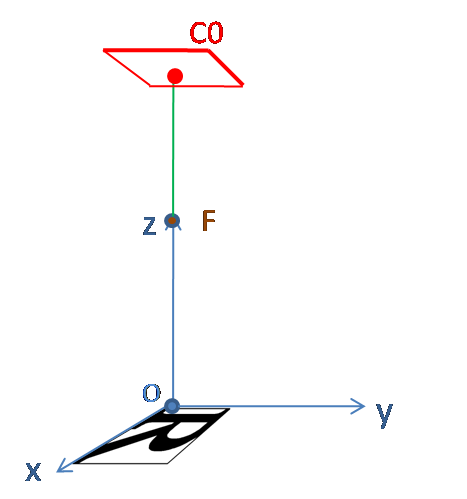
\includegraphics[scale=0.5]{vue_tps_identity.png}}}\\
		\subfigure[Vue après une première rotation (d'angle $\phi$)]{
		{
\includegraphics[width=60mm]{vue_fps_rotation_phi.png}}
		{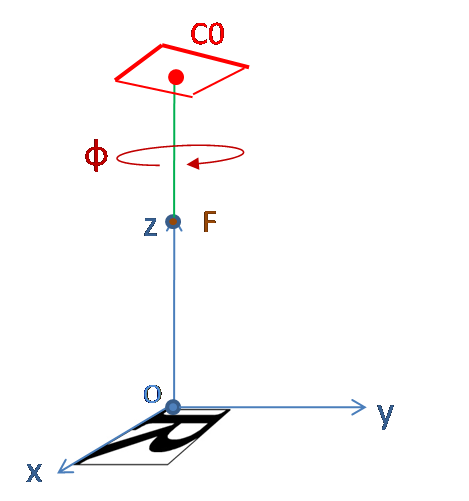
\includegraphics[scale=0.5]{vue_tps_rotation_phi.png}}}\\
		\subfigure[Vue après l'homographie unidirectionnelle]{
		{
\includegraphics[width=60mm]{vue_fps_hom_part.png}}
		{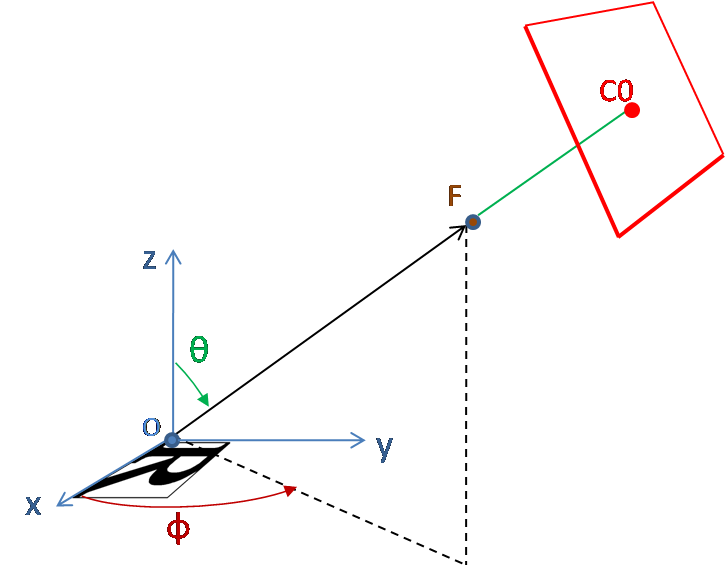
\includegraphics[scale=0.5]{vue_tps_hom_part.png}}}\\
		\subfigure[Vue finale (après rotation d'angle $\psi$)]{
		{
\includegraphics[width=60mm]{vue_fps_rotation_psi.png}}
		{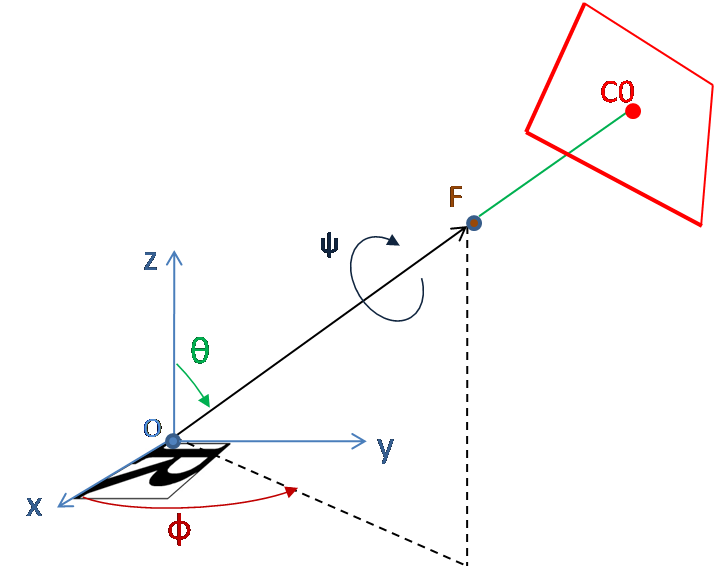
\includegraphics[scale=0.5]{vue_tps_rotation_psi.png}}}
		\caption{Étapes de traitement d'une homographie, assimilées à des mouvements de caméra, à gauche la vue de la caméra, à droite une vue extérieure immobile. Les translations ont été omise pour plus de clarté. Sur les vues extérieures, $F$ représente le point focal de la caméra, le plan rouge est le plan image de la caméra. (cf \ref{ref_schema_decomp_cool})}
		\label{schema_decomp_cool}
		\label{SchemaEtapesDecompoGeometrique}
	\end{figure}
\clearpage


































